% !TEX root = ../main.tex



\thispagestyle{empty}
\phantom{}\bigskip\bigskip

\begin{enumerate}

%
\begin{exercise}
% !TEX root = ../main.tex



 Beargumenteer het gebruik van het model van een eenparig versnelde beweging (EVB) voor de vrije beweging van een wagentje op een helling. Denk daarbij aan een proefneming die we in de klas deden. De notie kracht moet je hier even buiten beschouwing laten.

\begin{oplossing}

Het model beschrijft de meetgegevens accuraat.

M.a.w. zijn de meetgegevens van de positie van het wagentje op de helling in functie van de tijd, gemeten met een (ultrasone) positiesensor, accuraat te beschrijven met de plaatsfunctie van een eenparig versnelde beweging.

\emph{Toelichting}.
De vraag gaat over de relatie tussen de theorie en de realiteit. Het is maar door metingen te doen dat we kunnen nagaan of gevolgen van de theorie (in dit geval bijvoorbeeld dat de positie kwadratisch in de tijd verloopt voor een beweging met constante versnelling) overeenkomen met de realiteit. In het gegeven geval van een wagentje op een helling, is bijvoorbeeld een model van constante snelheid niet van toepassing. Het zou immers impliceren dat het wagentje niet van zin kan veranderen. Dat laatste wordt door metingen of waarnemingen weerlegd.

\end{oplossing} 

\end{exercise}
 % Model EVB wagentje op een helling
%
\begin{exercise}
% !TEX root = ../main.tex



 Wanneer de pelikaan naar vis duikt, trekt hij zijn vleugels in om als een steen loodrecht naar beneden te vallen. 

Stel een pelikaan duikt vanaf \SI{25}{m} hoogte en verandert onderweg dus niet meer van koers. Als het een vis \SI{0,15}{s} kost om te vluchten, wat is dan de hoogte waarop de vis de pelikaan minstens moet opmerken, wil de vis nog kans maken te ontsnappen? 

Neem aan dat de vis zich aan het wateroppervlak bevindt.

\begin{oplossing}
\item[Gegeven]$x_2=\SI{25}{m}$\newline$\Delta t=\SI{0,15}{s}$
\item[Gevraagd]$x_2-x_1$
\item[Oplossing]We kiezen de referentie-as naar beneden, met de oorsprong op de positie waar de pelikaan begint aan zijn duik. De versnelling is dan gelijk aan de valversnelling. 

We kennen de afstand waarover de pelikaan valt zodat we de tijd die de pelikaan nodig heeft om het wateroppervlak te bereiken, de valtijd, kunnen berekenen uit $x_2=\frac{1}{2}gt_2^2 $:
\begin{eqnarray*}
t_2=\sqrt{\frac{2x_2}{g}}
\end{eqnarray*}
De pelikaan heeft namelijk geen beginsnelheid.%De referentie-as is hierbij naar beneden gekozen, met de oorsprong daar waar de pelikaan begint te vallen.

Gedurende een tijd $t_1=t_2-\Delta t$ (15 honderdste van een seconde minder) mag de pelikaan vallen zonder door de vis te worden opgemerkt. De afstand boven het wateroppervlak is dan:
\begin{eqnarray*}
x_2-x_1&=&x_2-\frac{1}{2}gt_1^2\\
&=&x_2-\frac{1}{2}g\left(t_2-\Delta t\right)^2\\
%&=&x_2-\frac{1}{2}g\left(\sqrt{\frac{2x_2}{g}}-\Delta t\right)^2\\
%&=&\Delta t\sqrt{2gx_2}-\frac{1}{2}g\Delta t^2\\
&=&\SI{3,2}{m}
\end{eqnarray*}
\end{oplossing} 

\end{exercise}
 % Pelikaan die naar vis duikt
%
\begin{exercise}
% !TEX root = ../main.tex



\pt{10}Een parachutist in vrije val bereikt een uiteindelijke valsnelheid van \SI{50}{m/s}. Neem aan
dat een geopende parachute voor een constante vertraging van \SI{30}{m/s^2} zorgt.\footnote{Dit is een heel ruwe benadering. In feite hangt de vertraging door de parachute namelijk af van de snelheid en is die afhankelijkheid bovendien voor grote snelheden sterker dan voor kleine.} Wil er bij het neerkomen geen kans op letsel bestaan, dan mag de landingssnelheid niet groter dan \SI{5,0}{m/s} zijn. 

Wat is de minimumhoogte voor het openen van de parachute?

\begin{oplossing}
\item[Gegeven]$v_0=\SI{50}{m/s}$\newline$a=\SI{-30}{m/s^2}$\newline$v=\SI{5,0}{m/s}$
\item[Gevraagd]$x$
\item[Oplossing]Aangezien we de versnelling en begin- en eindsnelheid kennen, kunnen we de tijd die nodig is om de eindsnelheid te bereiken, berekenen:
\begin{eqnarray*}
v=v_0+at&\Leftrightarrow&t=\frac{v-v_0}{a}
\end{eqnarray*}
De afgelegde afstand is dan met de gemiddelde snelheid te berekenen:
\begin{eqnarray*}
x&=&\overline{v}t\\
&=&\frac{v_0+v}{2}\cdot\frac{v-v_0}{a}\\
&=&\frac{v^2-v_0^2}{2a}\\
&=&\SI{41,25}{m}
\end{eqnarray*}
\end{oplossing}

\end{exercise}
 % Parachutist
%\input{./fy_files/dyn_ECB_II_1} % hiet is iets misgegaan. Dat bestand moet overschreven zijn geweest.

\item[Opgave]\begin{minipage}[t]{0.5\textwidth}
Welke snelheid moet een achtbaanwagentje dat op zijn kop boven in een lus aankomt ten minste hebben, willen de passagiers niet naar beneden vallen? Neem aan dat de kromtestraal van de lus $7,0\rm\,m$ bedraagt.
\end{minipage}
\hspace{5mm}
\begin{minipage}[t]{0.45\textwidth}
\raisebox{-2cm}{
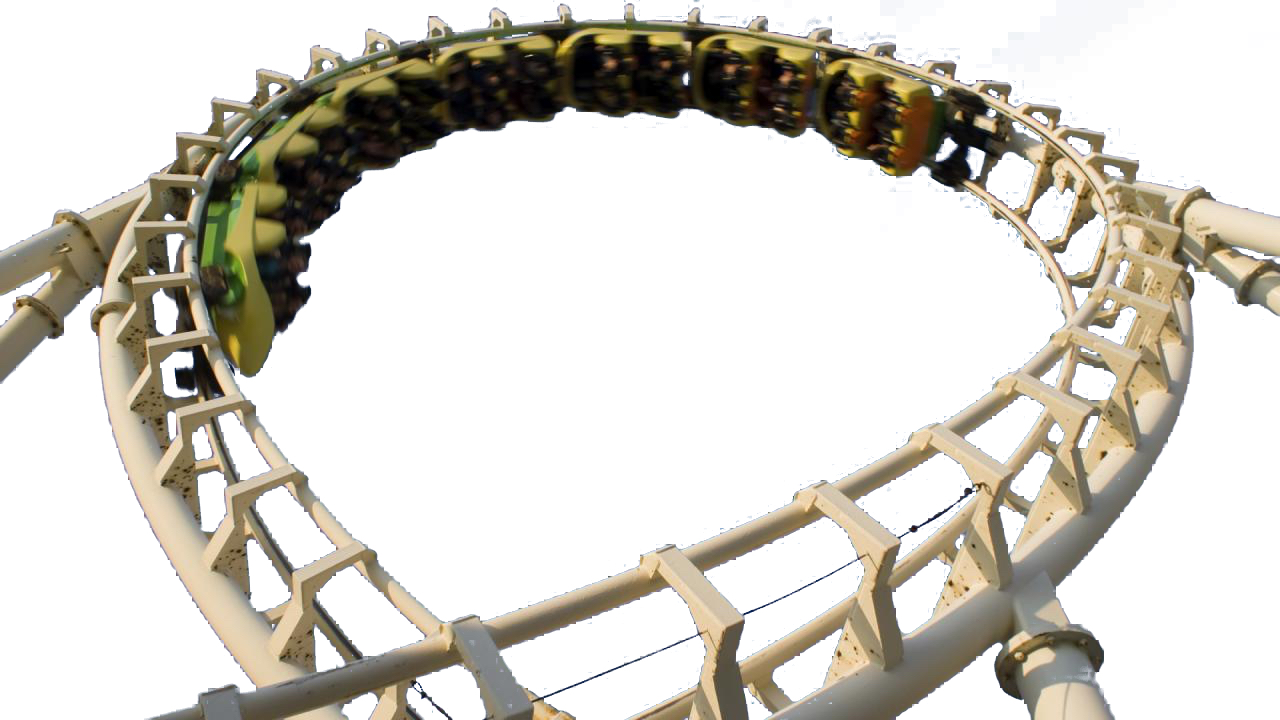
\includegraphics[width=0.9\textwidth]{gewonden-ontsporing-achtbaan-vs_res}
}
\end{minipage}


\begin{oplossing}
De snelheid moet groot genoeg zijn zodat de zwaartekracht er niet in slaagt de passagiers sneller uit de bocht te trekken dan noodzakelijk. Hoe trager de passagiers gaan, hoe minder groot de middelpuntzoekende kracht moet zijn om die beweging tot stand te brengen. 
\newline
Bij een snelheid die groot genoeg is, helpt de normaalkracht (door de wagentjes op de passagiers uitgeoefend) de zwaartekracht om een middelpuntzoekende kracht te genereren. De minimale snelheid vinden we dan ook wanneer de normaalkracht wegvalt en enkel de zwaartekracht de middelpuntzoekende kracht levert:
\begin{eqnarray*}
		F=ma\Rightarrow mg=\frac{mv^2}{r}
\end{eqnarray*}
Zodat:
$v_{\rm min}=\sqrt{rg}=8,29\rm\,m/s=29,8\rm\,km/h$.
\end{oplossing}

\end{enumerate}